\documentclass[a4paper,twoside,10pt,french,twocolumn]{scrartcl}
\usepackage{amsthm}
\usepackage{amsmath}
\usepackage[T1]{fontenc}
\usepackage{graphicx}
\usepackage{titlesec}
\usepackage{ulem}
\usepackage[dvipsnames]{xcolor}
\usepackage{color}
\usepackage{amssymb}
\usepackage{caption}
\usepackage[mathscr]{euscript}
\usepackage{babel} 
\usepackage{helvet} 
\usepackage[utf8]{inputenc}
\usepackage[T1]{fontenc}
\usepackage{geometry}
\title{Application du produit scalaire}
\date{}
 \renewcommand*\familydefault{\sfdefault} 
\geometry{a4paper}
% -------------------------------------------------------------------------------------------------
% ----------- Création des commandes de couleur pour les titres ----------
% -------------------------------------------------------------------------------------------------
\newcommand{\sectionred}[1]{{\color{red}{\uuline{\color{black}#1}}}}
\newcommand{\sectiongreen}[1]{{\color{ForestGreen}{\uuline{\color{black}#1}}}}
\newcommand{\sectionblue}[1]{{\color{NavyBlue}{\uuline{\color{black}#1}}}}
\begin{document}
\maketitle
% -------------------------------------------------------------------------------------------------
% ---------------- Modification des titres de niveau 1,2 et 3 --------------------
% -------------------------------------------------------------------------------------------------
\titleformat
{\section} % command
%[display] % shape
{\Large} % format
{{\color{red}\uuline{\color{black}\thesection -}}} % label
{0ex} % sep
{\sectionred} % before-code
[] % after-code

\titleformat
{\subsection}%[display] % shape
{\Large} % format
{{\color{ForestGreen}\uuline{\color{black}\thesubsection -}}} % label
{0ex} % sep
{\sectiongreen} % before-code
[] % after-code

\titleformat
{\subsubsection} % command
%[display] % shape
{\large} % format
{{\color{NavyBlue}\uuline{\color{black}\thesubsubsection -}}} % label
{0ex} % sep
{\sectionblue} % before-code
[] % after-code

% -------------------------------------------------------------------------------------------------
% ---------------- Début du corps du document ------------------------------------
% -------------------------------------------------------------------------------------------------

\section{Formule\:d'Al-Kashi}
On considère le triangle suivant :

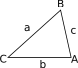
\includegraphics[scale=0.2]{fig-1}

Relations :
\begin{itemize}
 \item $a^2 = b^2+c^2 - 2 \times b \times c \times \cos (\widehat{A})$
 \item $b^2 = a^2+c^2 - 2 \times a \times c \times \cos (\widehat{B})$
 \item $c^2 = b^2+a^2 - 2 \times b \times a \times \cos (\widehat{C})$
\end{itemize}

\section{Transformation\:de\:$\protect\overrightarrow{MA} \cdot \protect\overrightarrow{MB}$}
\subsection{Propriété\:et\:démonstration}
$A$ et $B$ sont 2 points et $I$ est le milieu de [AB].
\begin{proof}
\begin{align*}
	\overrightarrow{MA} \cdot \overrightarrow{MB} &=(\overrightarrow{MI} + \overrightarrow{IA}) \cdot (\overrightarrow{MI} + \overrightarrow{IB})\\
	 &= MI^2 + \overrightarrow{MI} \cdot \overrightarrow{IB} + \overrightarrow{IA} \cdot \overrightarrow{MI} + \overrightarrow{IA} \cdot \overrightarrow{IB}\\
	 &= MI^2 + \overrightarrow{MI} (\overrightarrow{IB} + \overrightarrow{IA}) - IA \times IB\\
	 &= MI^2 + \overrightarrow{MI} \cdot \overrightarrow{0} - IA \times IB\\
	 &= MI^2 - IA \times IB\\
	 &= MI^2 - \frac{AB}{2} \times \frac{AB}{2}\\
	 &= MI^2 - \frac{AB \times AB}{2 \times 2}\\
	 &= MI^2 - \frac{AB^2}{4}\\
\end{align*}
\end{proof}
\subsection{Trouver\:un\:ensemble\:de\:points}
On cherche l'ensemble de points tels que $\protect\overrightarrow{MA} \cdot \protect\overrightarrow{MB} = 2$. On sait que $AB = 8$.
\begin{align*}
	\protect\overrightarrow{MA} \cdot \protect\overrightarrow{MB} = 2 &\Longleftrightarrow\\
	 &\Longleftrightarrow MI^2 - \frac{AB^2}{4} = 2\\
	 &\Longleftrightarrow MI^2 - \frac{AB^2}{4} -2 = 0\\
	 &\Longleftrightarrow - \frac{AB^2}{4} -2 = - MI^2\\
	&\Longleftrightarrow \frac{AB^2}{4} +2 = MI^2\\
	&\Longleftrightarrow \frac{8^2}{4} +2 = MI^2\\
	&\Longleftrightarrow \frac{64}{4} +2 = MI^2\\
	&\Longleftrightarrow 16 +2 = MI^2\\
	&\Longleftrightarrow 18 = MI^2\\
	&\Longleftrightarrow \sqrt{18} = MI\\
\end{align*}
L'ensemble de points est le cercle de centre I et de rayon $MI = \sqrt{18}$.

\subsection{Remarques}
\begin{itemize}
 \item L'ensemble de points tels que $\protect\overrightarrow{MA} \cdot \protect\overrightarrow{MB} = 0$ est le cercle de centre I et de rayon $\frac{AB}{2}$.
 \item Si $M \in $ au cercle de diamètre [AB], alors $ABM$ est un triangle rectangle en $M$.
\end{itemize}
\section{Équation\:de\:droites}
\subsection{Rappels}
\begin{itemize}
 \item Une équation cartésienne d'une droite est de la forme $ax+by+c = 0$.
 \item Un vecteur directeur d'une droite est $\overrightarrow{u}(-b ; a)$.
  \item La longueur du vecteur $\overrightarrow{AB}$ ou du segment [AB] est $\sqrt{(x_B-x_A)^2+(y_B-y_A)^2}$ dans un repère orthonormé.
  \item Le vecteur $\overrightarrow{AB}$ a pour coordonnées $\overrightarrow{AB}(x_B-x_A ; y_B-y_A)$
  Les coordonnées du point $I$, mileu de [AB] sont $I(\frac{x_B+x_A}{2} ; \frac{y_B+y_A}{2})$
\end{itemize}
\subsection{Vecteur\:normal}
\begin{itemize}
\item Un vecteur est dit normal à une droite s'il est $\perp $ à celle-ci.
\item Un vecteur normal d'une droite est $\overrightarrow{n}(a ; b)$.
\item Pour trouver une équation cartésienne de droite avec un vecteur normal, on remplace $a$ et $b$ par les valeurs du vecteur normal, puis on résoud l'équation avec les coordonnées d'un point appartenant à cette droite (donné) pour trouver $c$.
\end{itemize}
\subsection{Projeté\:orthogonal}
On peut calculer les coordonnées du projeté orthogonal d'un point sur une droite.
\begin{enumerate}
\item On calcule l'équation de droite de la droite sur laquelle on projette le point.
\item On calcule l'équation de droite de la droite perpendiculaire à la droite avec le vecteur normal et les coordonnées du point projeté
\item Les coordonnées du point projeté sont la solution du système d'équation à deux inconnues fait par les 2 équations de droites trouvées dans les étapes précédentes
\end{enumerate}
\section{Équation\:de\:cercles}
\subsection{Forme\:traditionnelle}
Une équation cartésienne de cercle est $ (x-x_A)^2 + (y-y_A)^2 = r^2$ avec $x_A$ et $y_A$ les coordonnées du centre et $r$ le rayon.
\subsection{Forme\:secondaire}
Un cercle admet une équation cartésienne de la forme $x^2+y^2+ax+by+c = 0$.

Cependant, toutes les équations de cette forme ne sont pas des équations de cercle.
\subsection{Forme\:secondaire\:vers\:traditionnelle}
On utilise la méthode de la complétion du carré (déjà utilisée pour trouver la forme canonique d'une fonction du 2nd degrés)
\begin{enumerate}
 \item On a l'équation de la forme $x^2+y^2 +ax+by+c = d$
 \item On transforme $x^2 + ax$ en $ (x + \frac{a}{2})^2 - (\frac{a}{2})^2$. On fait de même pour les $y$.
 \item On obtient $(x + \frac{a}{2})^2 - (\frac{a}{2})^2 + (y + \frac{b}{2})^2 - (\frac{b}{2})^2 + c =d$.
 \item On fait passer $c, -(\frac{a}{2})^2$ et $-(\frac{b}{2})^2$ de l'autre côté.
 \item On obtient $(x + \frac{a}{2})^2 + (y + \frac{b}{2})^2 = (\frac{a}{2})^2 + (\frac{b}{2})^2 - c + d$.
\end{enumerate}

\end{document}
